% This version of CVPR template is provided by Ming-Ming Cheng.
% Please leave an issue if you found a bug:
% https://github.com/MCG-NKU/CVPR_Template.

% \documentclass[review]{cvpr}
\documentclass[final]{cvpr}

\usepackage{times}
\usepackage{epsfig}
\usepackage{graphicx}
\usepackage{amsmath}
\usepackage{amssymb}

% Include other packages here, before hyperref.

% If you comment hyperref and then uncomment it, you should delete
% egpaper.aux before re-running latex.  (Or just hit 'q' on the first latex
% run, let it finish, and you should be clear).
\usepackage[pagebackref=true,breaklinks=true,colorlinks,bookmarks=false]{hyperref}

%\setcounter{page}{4321} % For final version only


\begin{document}

%%%%%%%%% TITLE
\title{Image Processing and Computer Vision (CSC6051/MDS6004)  \\ Assignment 1}

\author{Your Name\\
Your Student ID\\
{\tt\small youremailaddress@link.cuhk.edu.cn}
}

\maketitle


%%%%%%%%% ABSTRACT
\begin{abstract}
This report covers three tasks: (1) an affine image transformation implemented with explicit scale/rotation/translation; (2) a simple 3D-to-2D perspective projection pipeline to render a projected cube using a camera intrinsic matrix; and (3) portrait segmentation on EG1800. For Task~3, a UNet baseline reaches best validation pixel accuracy 0.9679, while an improved DeepLabV3-ResNet50 model with pretrained backbone, data augmentation, CE+Dice loss, and cosine LR schedule reaches 0.9797. We also implement a face-aware preprocessing option and demonstrate SAM2 zero-shot segmentation using a box prompt.
\end{abstract}

%-------------------------------------------------------------------------
\section{Task 1}

\paragraph{Implementation Details}
We implement an affine transformation function that applies scaling, rotation, and translation to an input image. Concretely, three non-collinear source points are selected from the image corners, then we compute their destination locations by rotating/scaling around the image center and translating by $(t_x,t_y)$. The affine matrix $\mathbf{M}\in\mathbb{R}^{2\times3}$ is obtained with \texttt{cv2.getAffineTransform}, and the image is warped using \texttt{cv2.warpAffine} (bilinear interpolation with constant border).


\paragraph{Results \& Analysis}
Fig.~\ref{fig:task1_affine} shows a qualitative example of the affine transform output.

\begin{figure}[t]
   \centering
   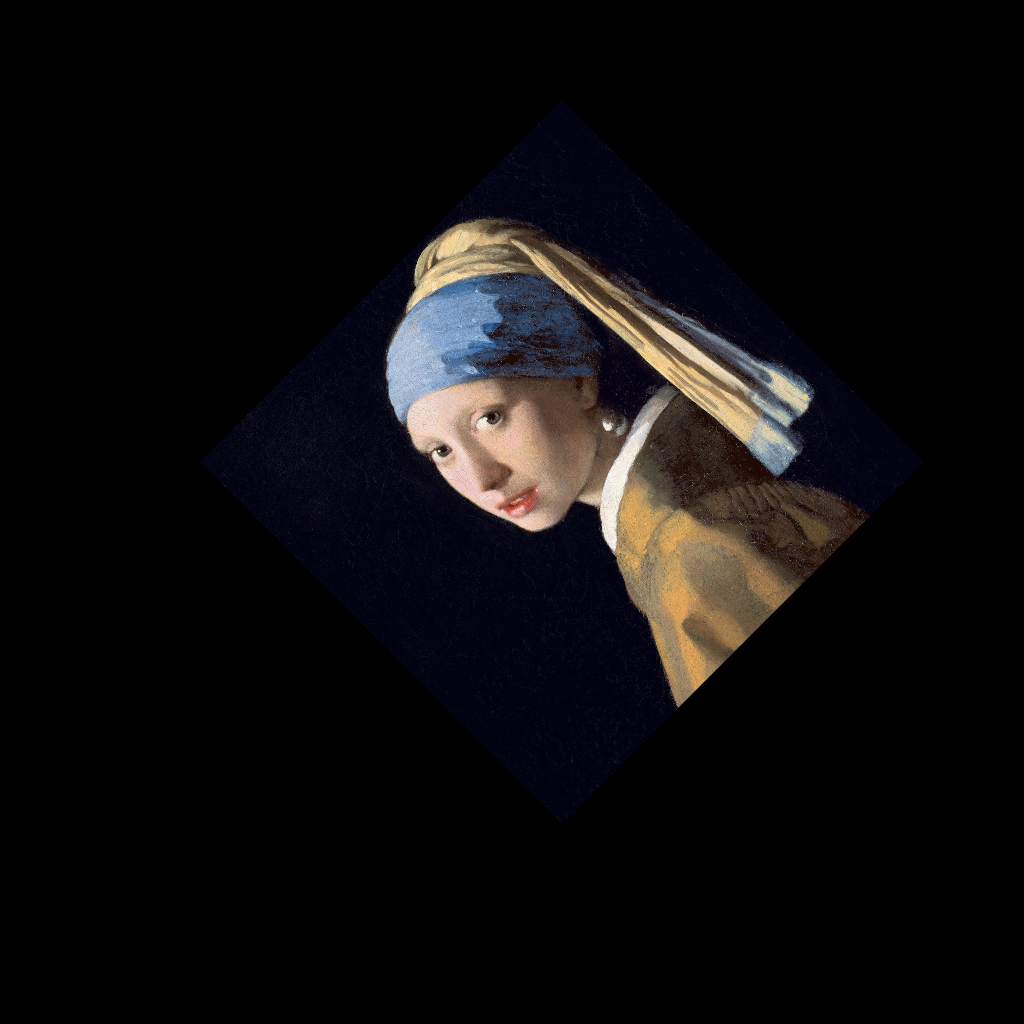
\includegraphics[width=0.95\linewidth]{../results/affine_result.png}
   \caption{Task 1: Example affine transformation result (scale/rotation/translation).}
   \label{fig:task1_affine}
\end{figure}


%-------------------------------------------------------------------------
\section{Task 2}

\paragraph{Implementation Details}
This task implements a minimal camera model and perspective projection. The camera intrinsics are
\begin{equation}
\mathbf{K} =
\begin{bmatrix}
\alpha & 0 & c_x\\
0 & \beta & c_y\\
0 & 0 & 1
\end{bmatrix},
\end{equation}
and a 3D point in camera coordinates $\mathbf{x}_c=(X,Y,Z)$ is projected to pixel coordinates using
\begin{equation}
\tilde{\mathbf{u}} = \mathbf{K}\,\mathbf{x}_c,\quad
\mathbf{u} = \left(\frac{\tilde{u}_x}{\tilde{u}_z},\frac{\tilde{u}_y}{\tilde{u}_z}\right).
\end{equation}
We generate a cube mesh (6 faces, 8 corners), apply 3D rotation (Euler angles) and translation, project all vertices to 2D, and visualize each face as a filled polygon.


\paragraph{Results \& Analysis}
Fig.~\ref{fig:task2_cube} shows projected cubes with different poses/locations.

\begin{figure}[t]
   \centering
   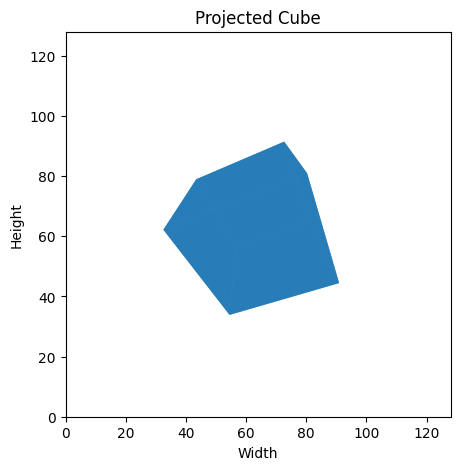
\includegraphics[width=0.32\linewidth]{../results/task2_1.png}
   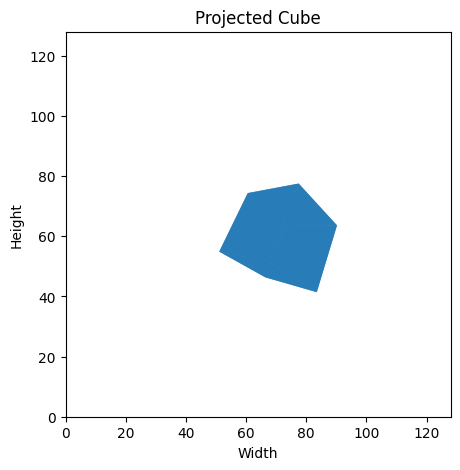
\includegraphics[width=0.32\linewidth]{../results/task2_2.png}
   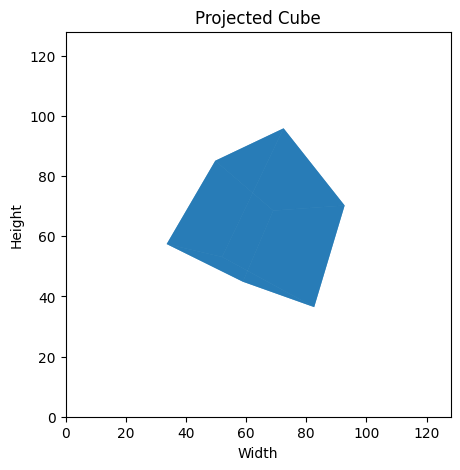
\includegraphics[width=0.32\linewidth]{../results/task2_3.png}
   \caption{Task 2: Projected cube renderings under different 3D rotations and translations.}
   \label{fig:task2_cube}
\end{figure}


%-------------------------------------------------------------------------
\section{Task 3}
\paragraph{Problem Setup}
We train a portrait segmentation model on the EG1800 dataset with two classes (background vs person). We report validation loss and pixel accuracy over 20 epochs, and save learning curves and prediction visualizations.

\paragraph{Baseline Model}
The baseline uses a UNet~\cite{ronneberger2015unet} trained with cross-entropy loss (input size 224, batch size 8, Adam optimizer with $\text{lr}=10^{-4}$).

\paragraph{Improved Model}
To improve performance, we switch to DeepLabV3-ResNet50~\cite{chen2017deeplab} from torchvision with a pretrained ResNet50 backbone, apply lightweight data augmentation, use CE+Dice loss, and adopt a cosine learning-rate schedule.

\paragraph{Face-aware Preprocessing}
We implement an optional face-aware crop: a Haar-cascade face detector proposes a face bounding box, then the image is cropped around the face with a margin and resized back to the network input resolution. This is designed to increase robustness when the face/person is not centered.

\paragraph{Zero-shot Segmentation with SAM2}
We run SAM2~\cite{sam2} in a zero-shot setting using a box prompt. The box is taken from the face detector when available; otherwise a default center box is used. We choose the best mask from SAM2's multimask outputs by the reported score.

\begin{figure*}[t]
   \centering
   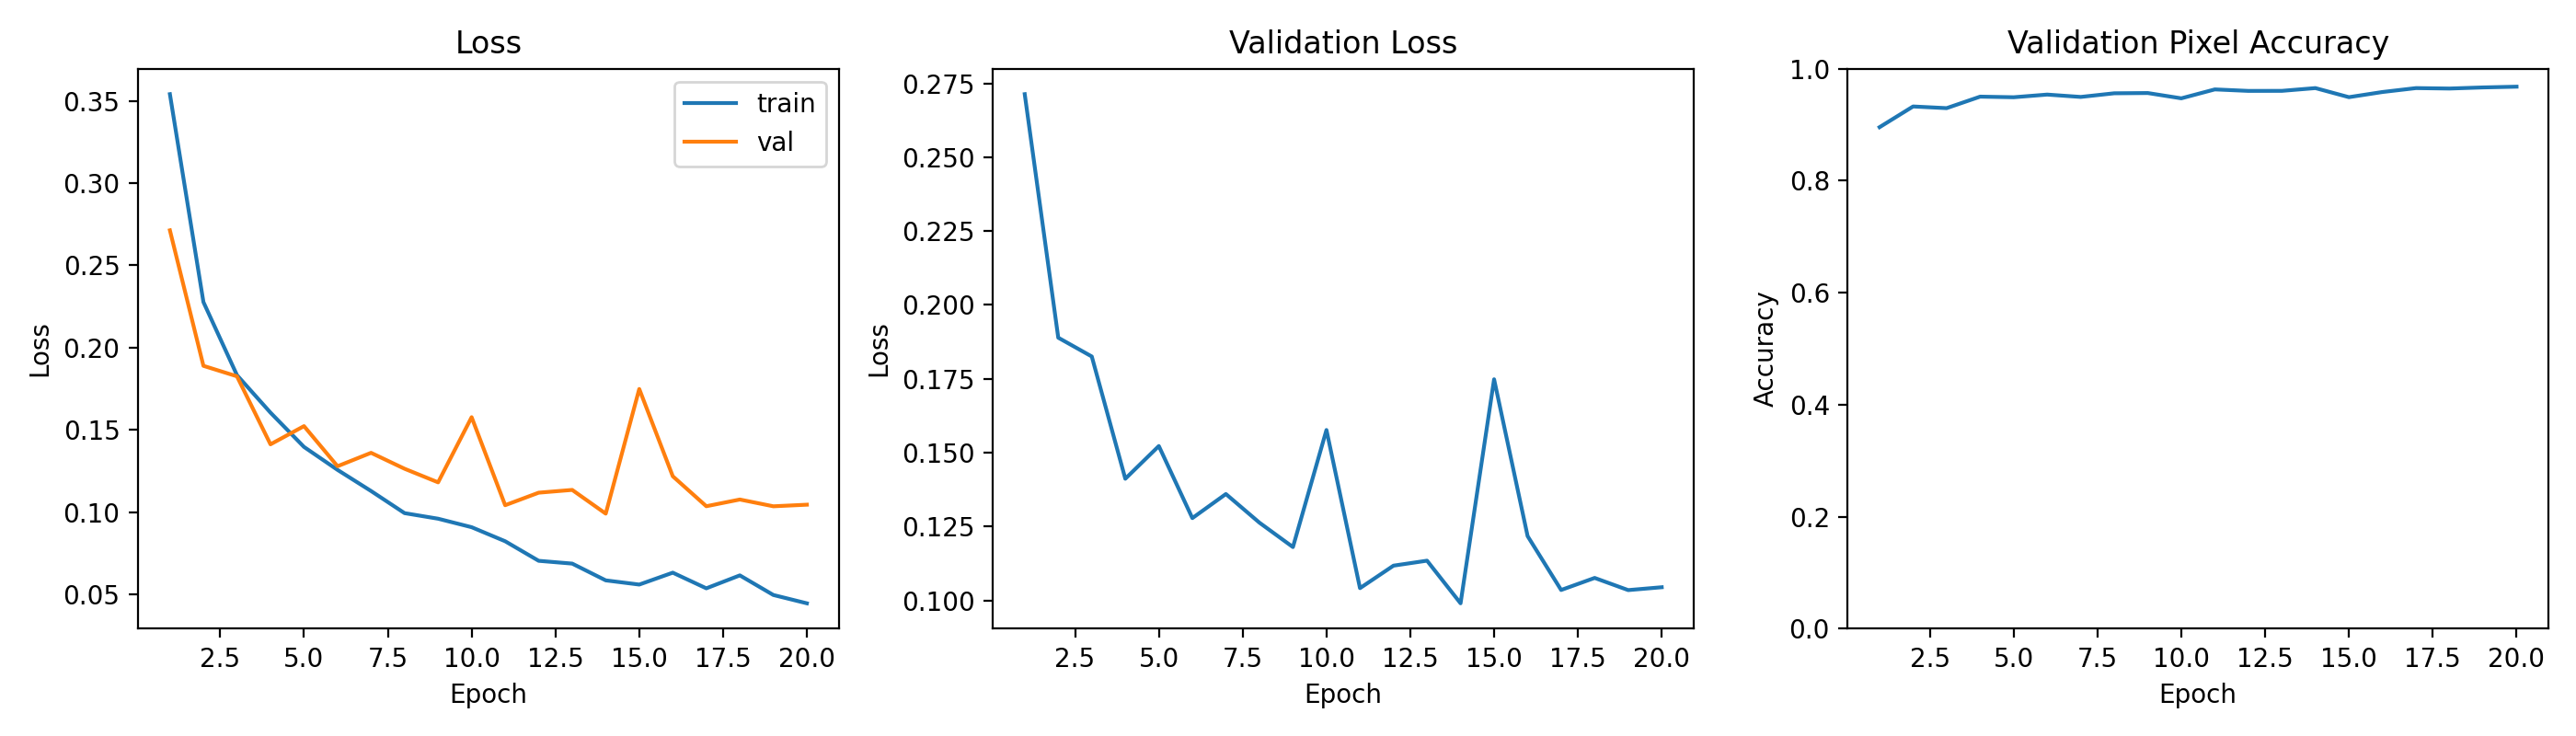
\includegraphics[width=0.32\linewidth]{../results/curves_baseline.png}
   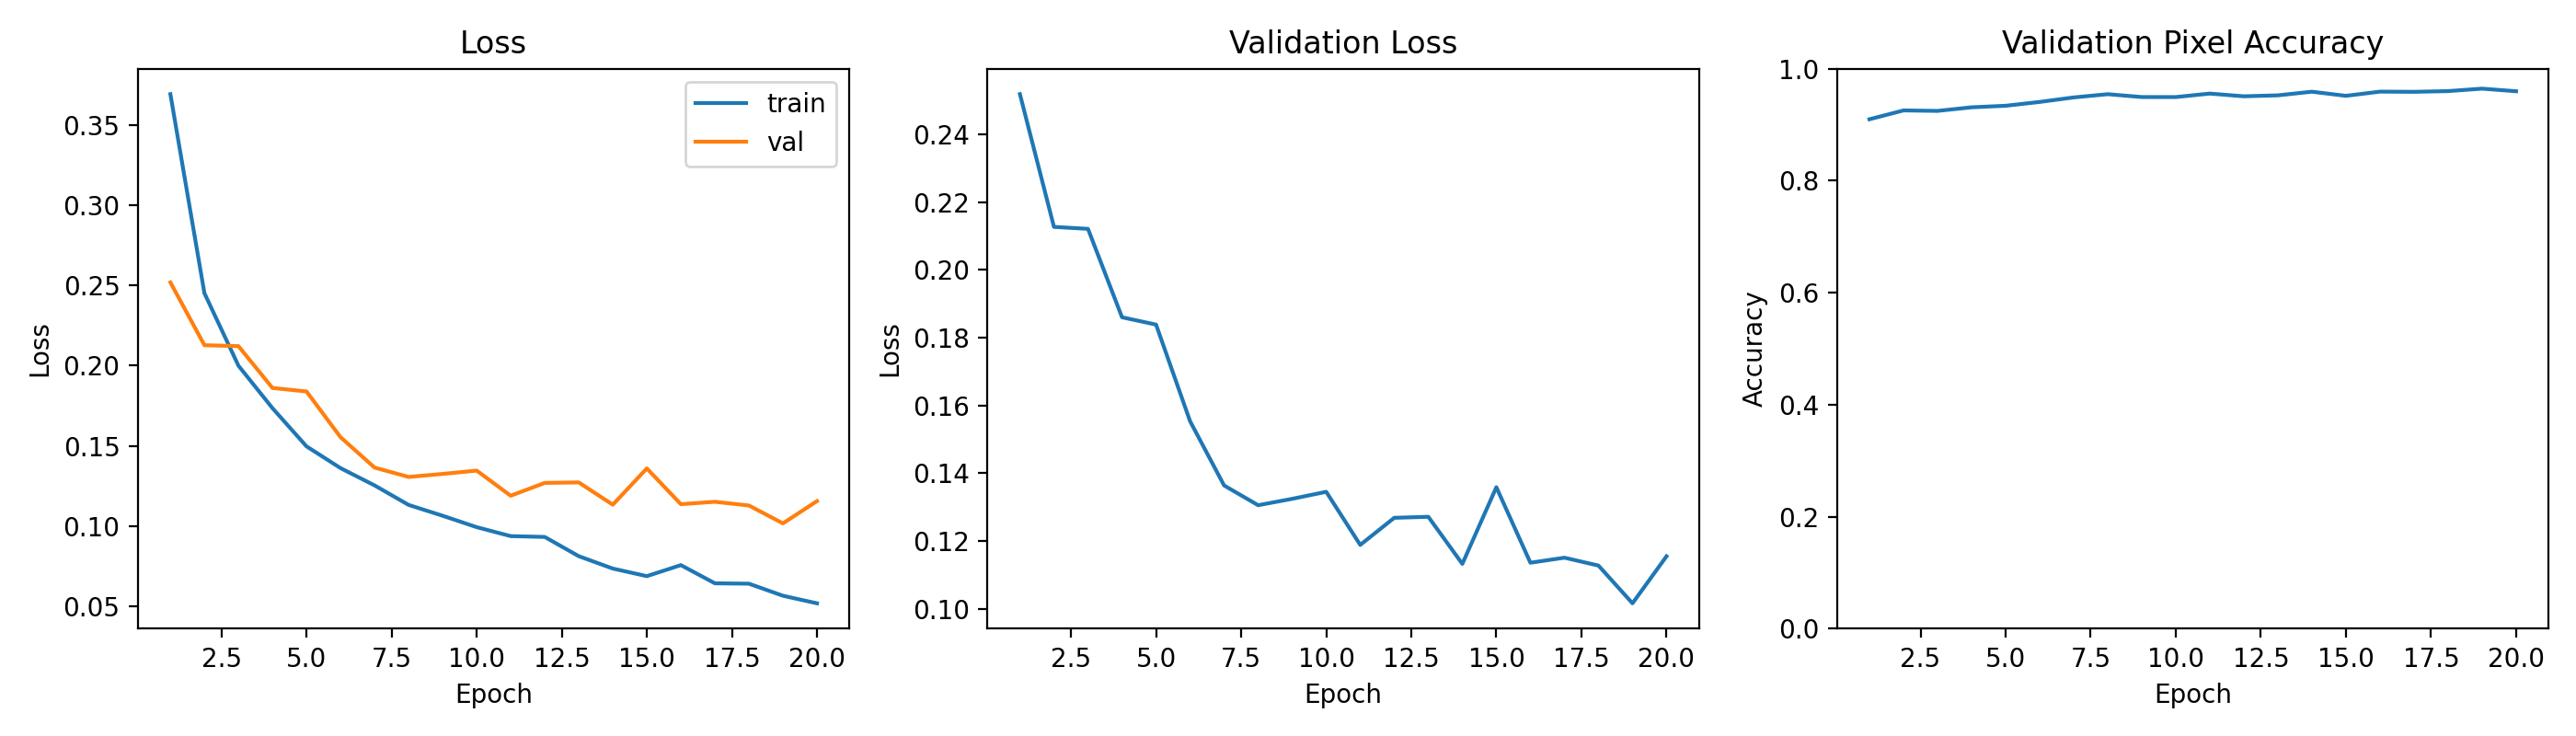
\includegraphics[width=0.32\linewidth]{../results/curves_facecrop.png}
   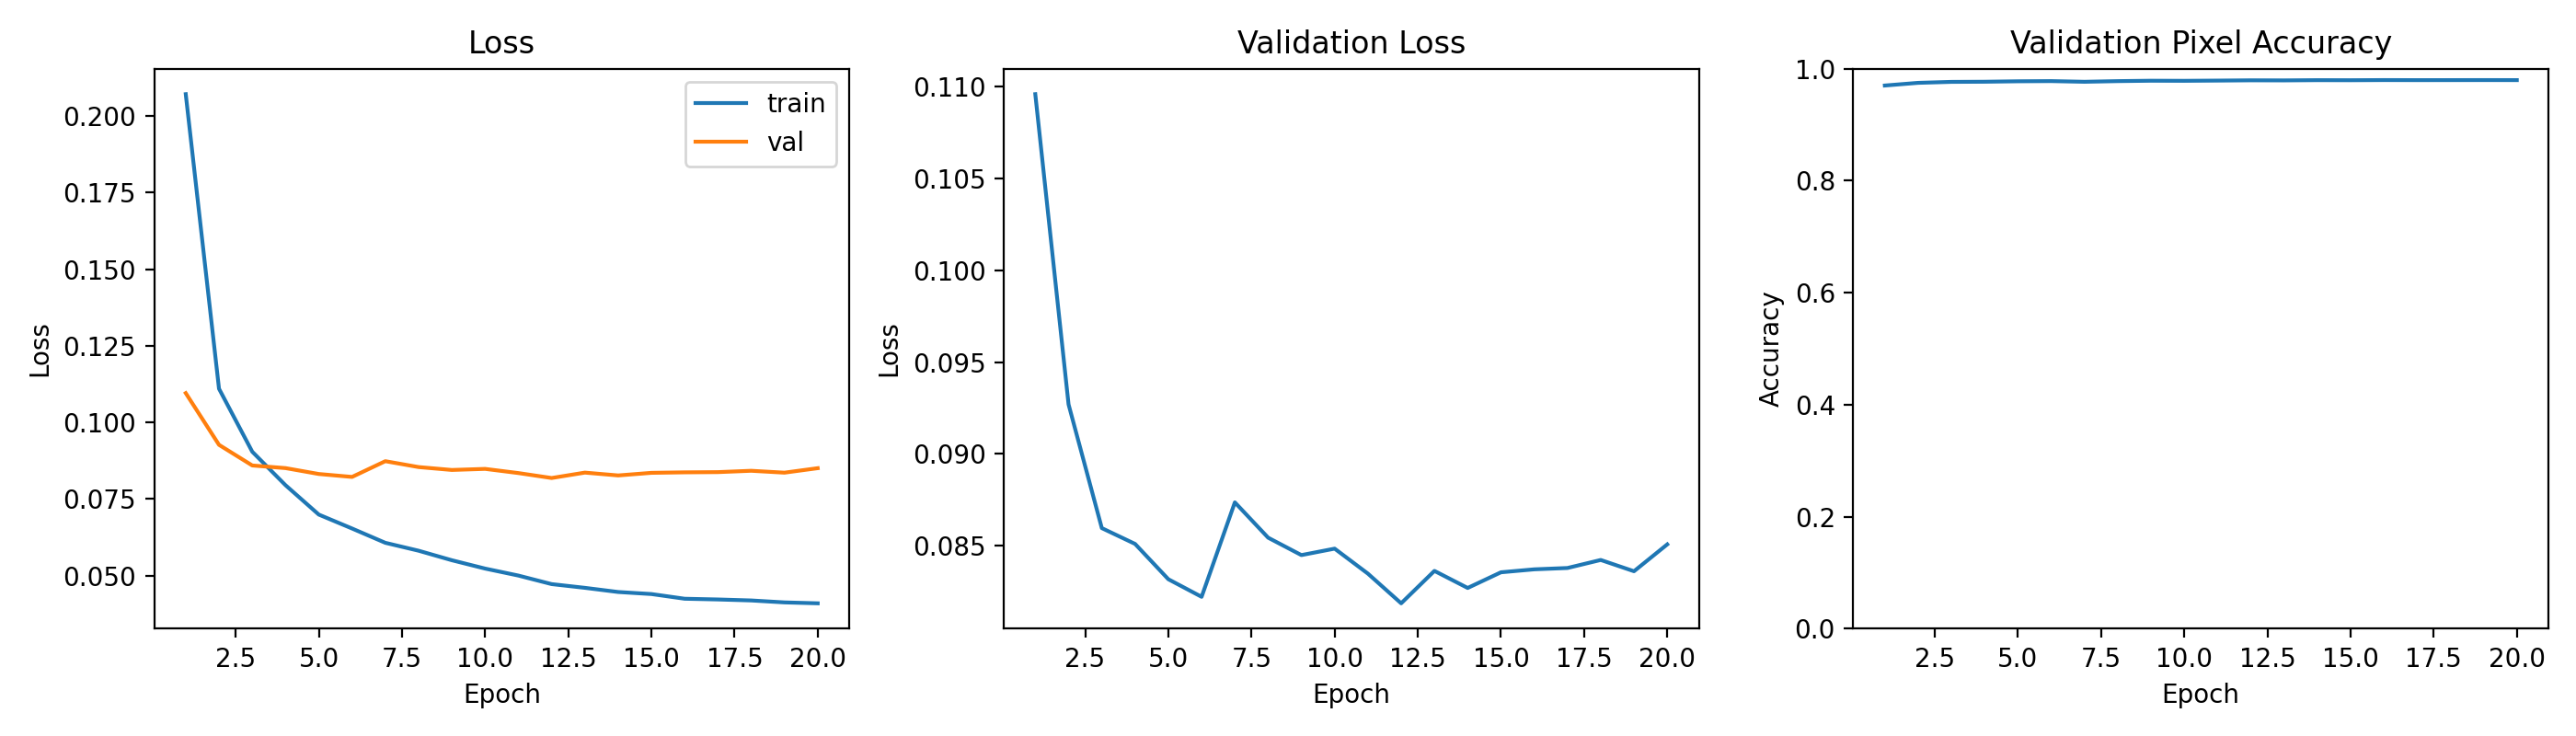
\includegraphics[width=0.32\linewidth]{../results/curves_improved.png}
   \caption{Task 3: Learning curves (train loss, val loss, val pixel accuracy). Left: UNet baseline. Middle: UNet + face-aware preprocessing. Right: improved DeepLabV3-ResNet50 with pretrained backbone, augmentation, CE+Dice, and cosine LR schedule.}
   \label{fig:task3_curves}
\end{figure*}

\begin{figure*}[t]
   \centering
   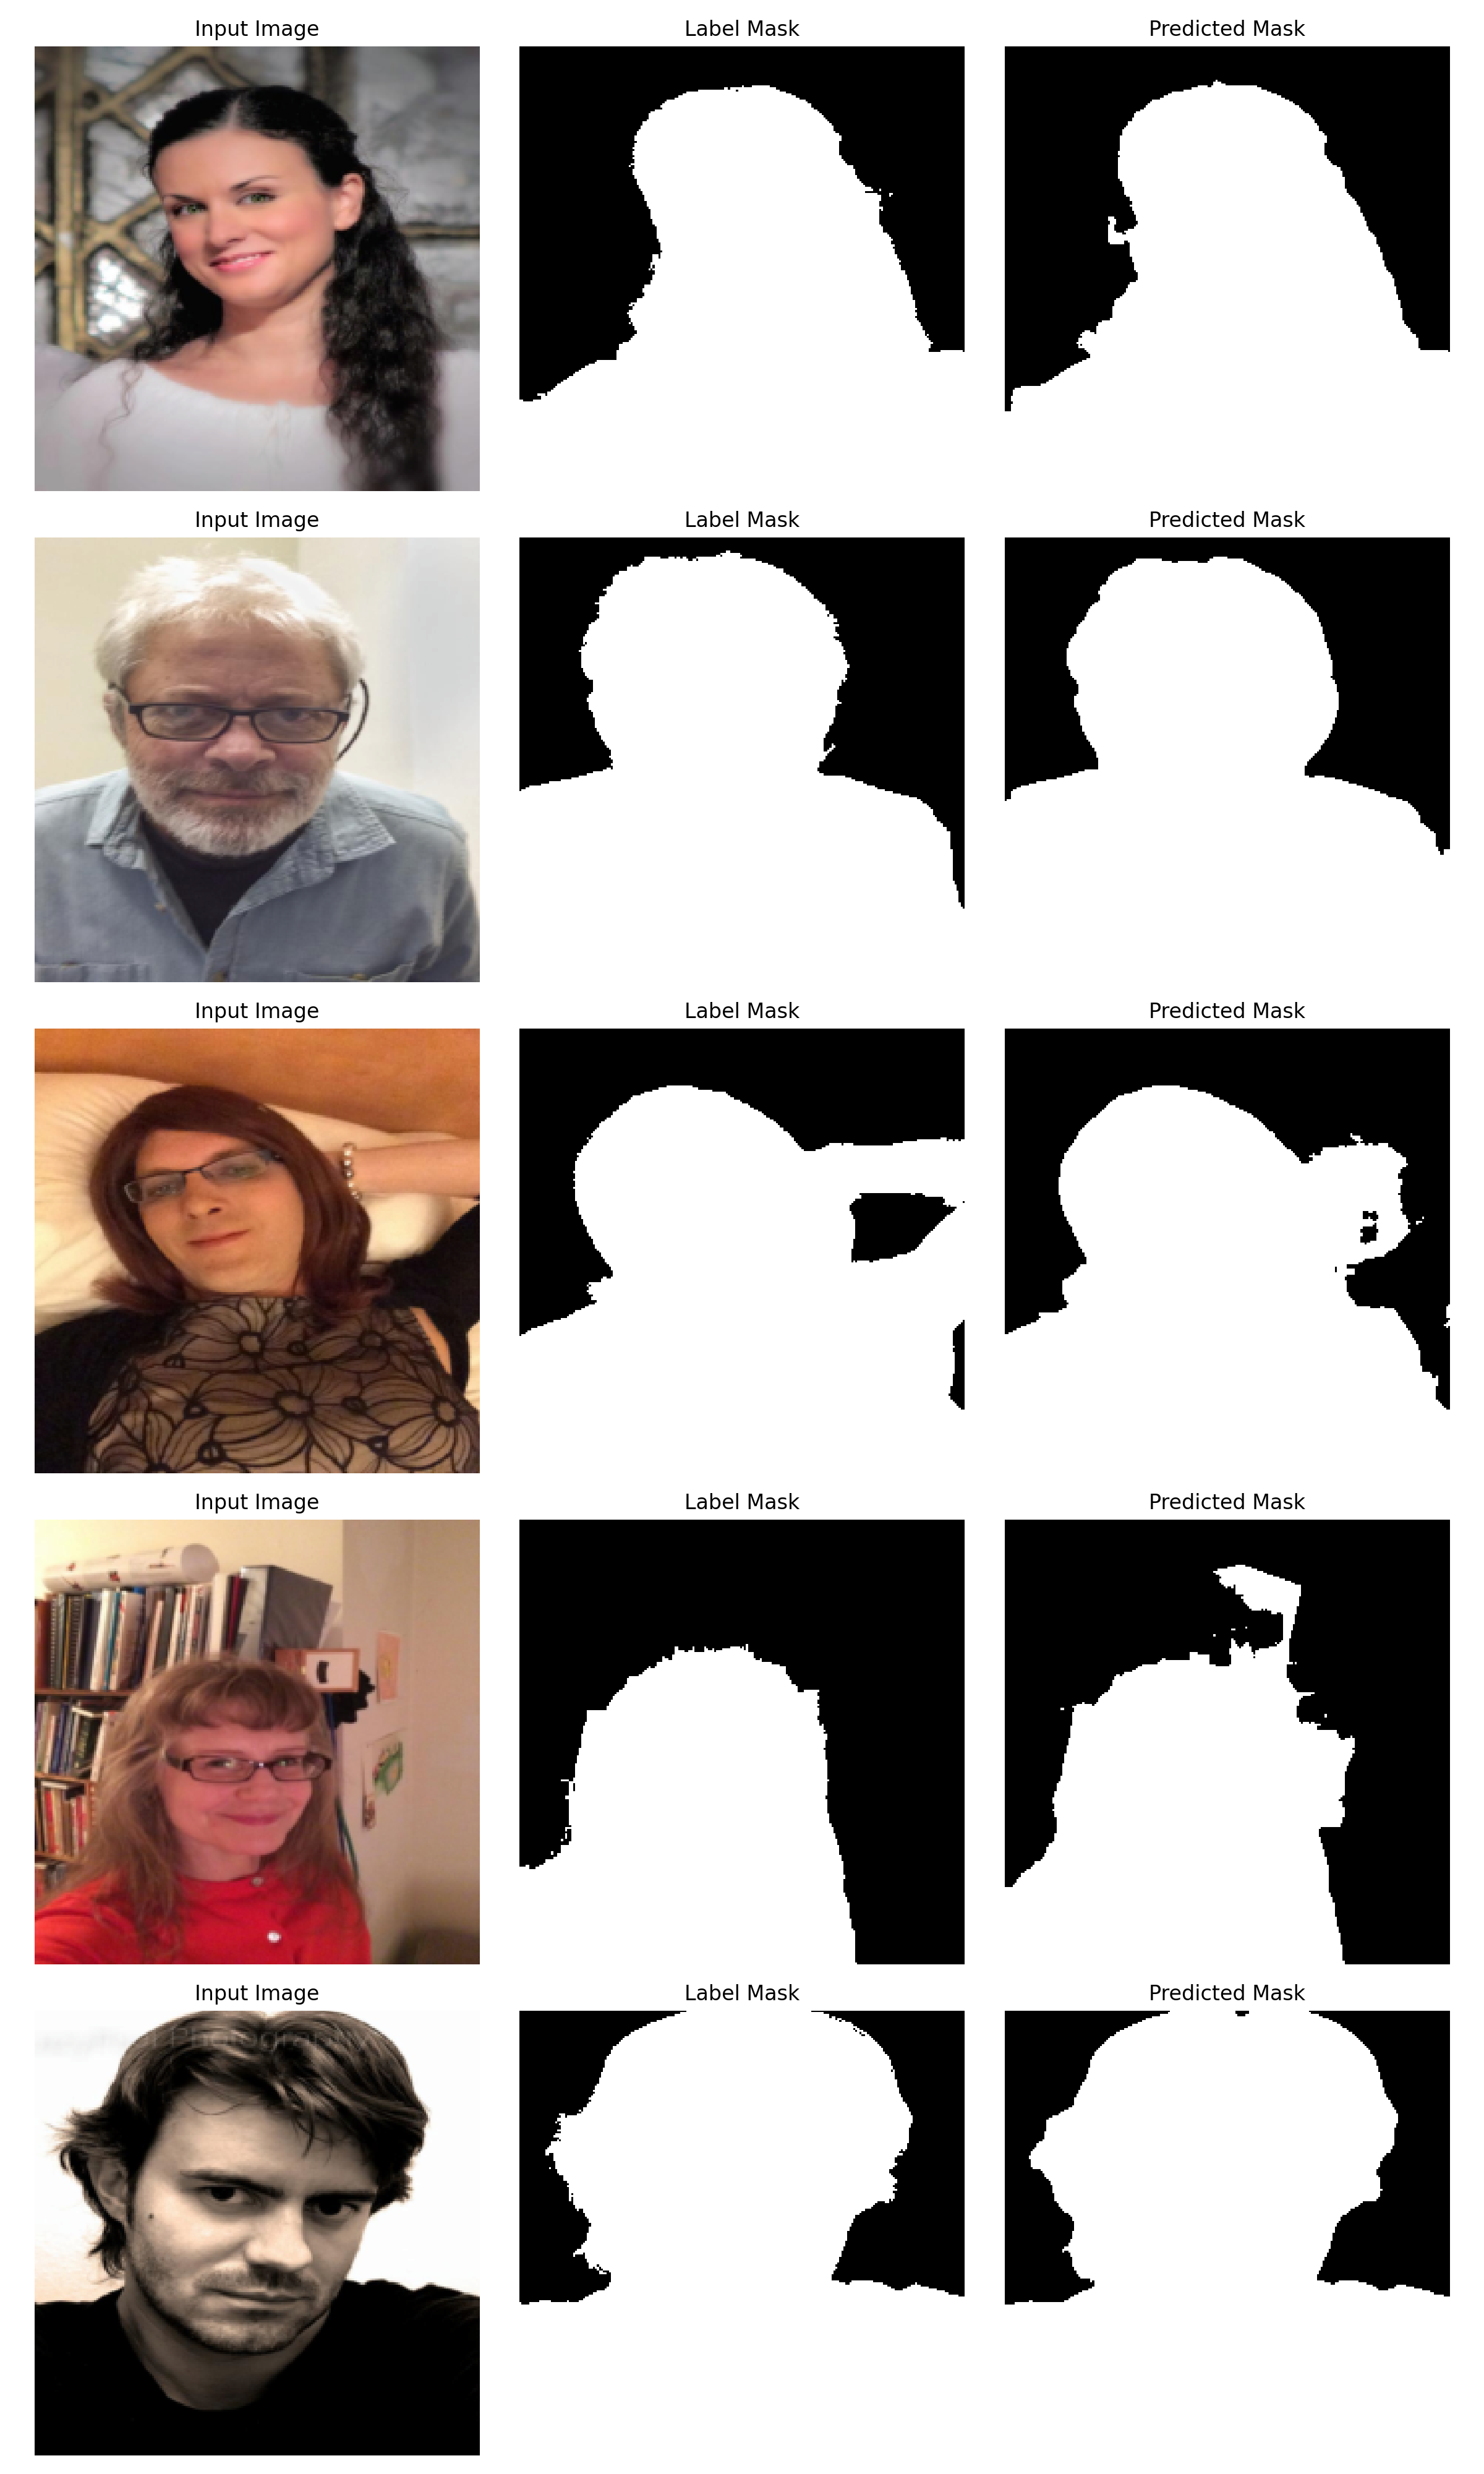
\includegraphics[width=0.48\linewidth]{../results/predictions.png}
   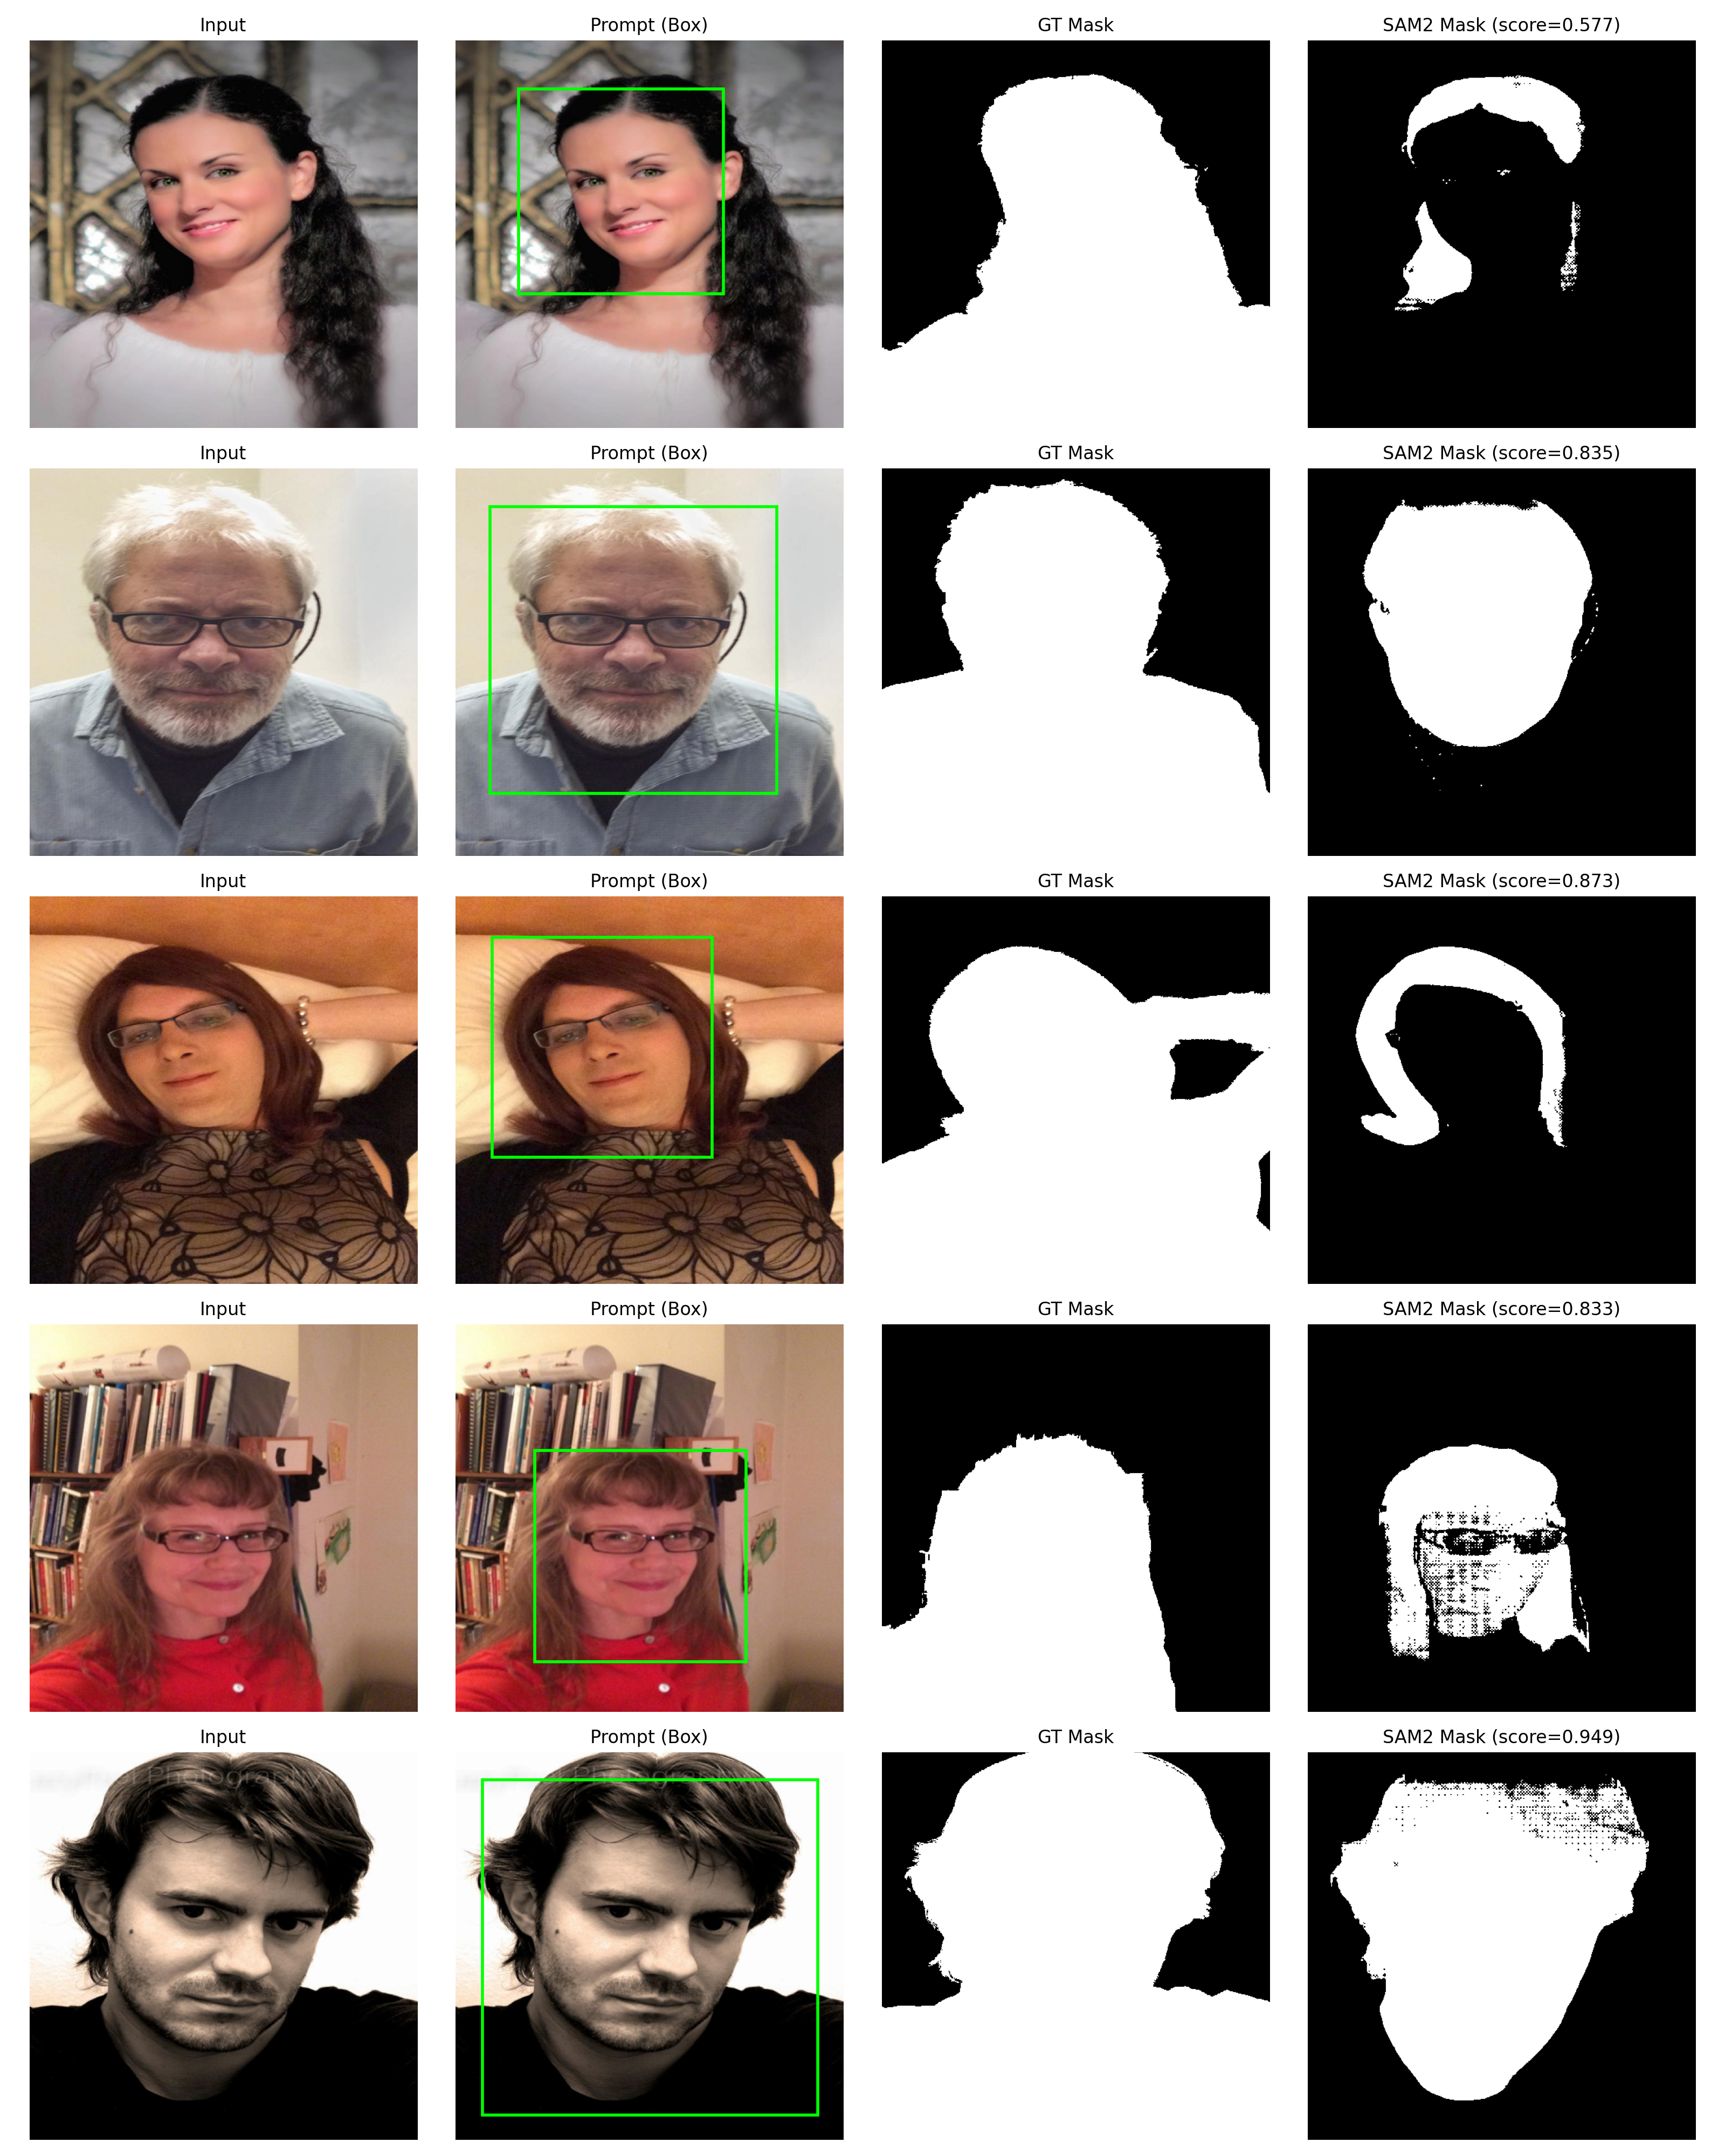
\includegraphics[width=0.48\linewidth]{../results/sam2_examples.png}
   \caption{Task 3: (Left) Model prediction visualization (input / ground-truth / predicted mask). (Right) SAM2 zero-shot examples showing the input, box prompt, ground-truth mask, and SAM2 mask.}
   \label{fig:task3_vis}
\end{figure*}


\begin{table}[htb]
\begin{center}
\begin{tabular}{|l|c|c|}
\hline
Method & Best Val Loss (epoch) & Best Val Pixel Acc (epoch) \\
\hline
UNet baseline & 0.0990 (14) & 0.9679 (20) \\
UNet + face-crop & 0.1016 (19) & 0.9644 (19) \\
DeepLabV3 (improved) & 0.0819 (12) & 0.9797 (16) \\
\hline
\end{tabular}
\end{center}
\caption{Task 3: Summary of best validation performance from \texttt{results/metrics\_*.json}.}
\end{table}

\section{Conclusion}
We implemented the required geometric transformations and projection pipeline (Tasks 1--2), and built a complete portrait segmentation pipeline for Task~3. The improved DeepLabV3 configuration achieves higher validation accuracy than the UNet baseline, and SAM2 provides competitive zero-shot masks with only a box prompt.

{\small
\bibliographystyle{ieee_fullname}
\bibliography{egbib}
}

\end{document}
